\documentclass[runningheads]{llncs}

\usepackage{tabularx}
\usepackage{booktabs}
\usepackage[export]{adjustbox}
\usepackage{array}
\newcolumntype{L}[1]{>{\raggedright\let\newline\\\arraybackslash\hspace{0pt}}p{#1}}
\newcolumntype{C}[1]{>{\centering\let\newline\\\arraybackslash\hspace{0pt}}p{#1}}
\newcolumntype{R}[1]{>{\raggedleft\let\newline\\\arraybackslash\hspace{0pt}}p{#1}}

% Used for displaying a sample figure. If possible, figure files should
% be included in EPS format.
\usepackage{graphicx}
\graphicspath{{../images/}}

% If you use the hyperref package, please uncomment the following line
% to display URLs in blue roman font according to Springer's eBook style:
\usepackage[colorlinks=true, linkcolor=blue, urlcolor=blue, citecolor=blue, anchorcolor=blue]{hyperref}
\renewcommand\UrlFont{\rmfamily}

\begin{document}

\title{Learning Grasp Evaluation Models Using Synthetic 3D Object-Grasp Representations}

%\titlerunning{Abbreviated paper title}
% If the paper title is too long for the running head, you can set
% an abbreviated paper title here
%
\author{
    Minh Nguyen \inst{1} \and
    Paul G. Pl\"{o}ger \and
    Alex Mitrevski\inst{1} \and
    Maximilian Sch\"{o}bel\inst{1}}
%
\authorrunning{M. Nguyen et al.}
% First names are abbreviated in the running head.
% If there are more than two authors, 'et al.' is used.
%
\institute{Hochschule Bonn-Rhein-Sieg, Grantham-Allee 20, 53757 Sank Augustin, Germany \\
\email{minh.nguyen@smail.h-brs.de}, \email{\{paul.ploeger,aleksandar.mitrevski,maximilian.schoebel\}@h-brs.de} \\
\url{www.h-brs.de}}
%
\maketitle              % typeset the header of the contribution
%
%\begin{abstract}
%The abstract should briefly summarize the contents of the paper in
%150--250 words.
%
%\keywords{First keyword  \and Second keyword \and Another keyword.}
%\end{abstract}
%

\section{Publishable Results}


\begin{table}[!h]
    \scriptsize
    \def\arraystretch{1.2}
    \begin{tabularx}{\linewidth}{L{0.05\linewidth}C{0.39\linewidth}L{0.28\linewidth}L{0.28\linewidth}}
        Method & Object-grasp\linebreak representation & Feature extraction \& learning model & Data generation \\
        \toprule
        \cite{jiang2011}    & 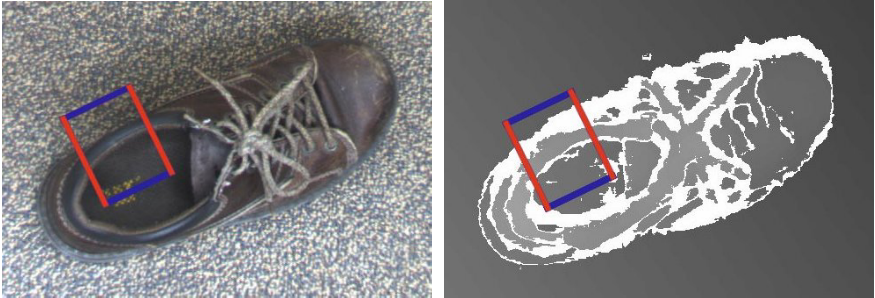
\includegraphics[scale=0.09,valign=t]{jiang_et_al-2011-grasp_representation}
        & Histogram of hand-crafted filters; \linebreak Model: SVM.
        & Rectangles manually \linebreak annotated. \\
        \cite{lenz2015}     & 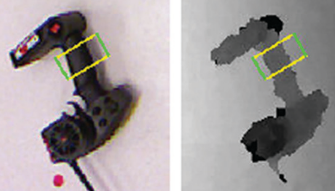
\includegraphics[scale=0.16,valign=t]{lenz_et_al-2015-grasp_representation}
        & Auto-encoders to initialize weights, structured regularization to combine depth
        and RGB data; \linebreak Model: MLP.
        & Extension of the \linebreak dataset from \cite{jiang2011} \linebreak (above).\\
        \cite{Kappler2015}  &
        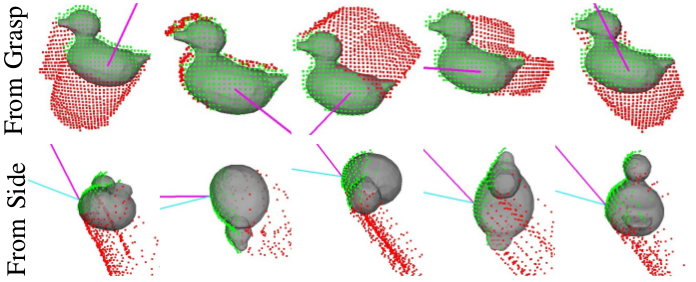
\includegraphics[scale=0.16,valign=t]{kappler_et_al-2015-fig8-local_shape_diff_viewpoints}
        & RGB rendering of ``template grids''; \linebreak Model: LeNet CNN
        & Quality of grasps are \linebreak calculated in simulation \linebreak for object
        meshes, \linebreak verified via crow-sourcing. \\
        \cite{Gualtieri2016}& 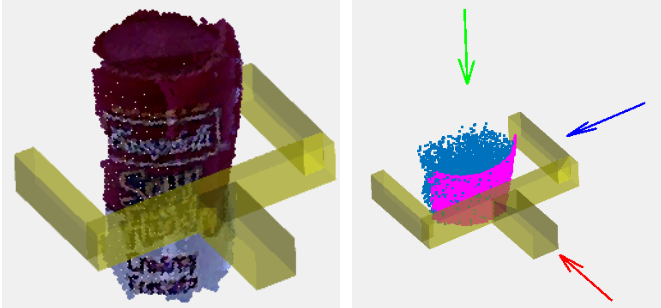
\includegraphics[scale=0.1,valign=t]{Gualtieri_et_al-2016-grasp_representation}
        & Filters of cuboid regions projected onto 3 orthogonal planes, creating 15 channels;
        \linebreak Model: LeNet CNN.
        & Quality of grasps are \linebreak calculated for object \linebreak meshes using
        force-closure \\
        \cite{mahler2017}   & 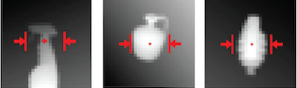
\includegraphics[scale=0.22,valign=t]{mahler_et_al-2017-grasp_representation}
        & Depth images cropped and aligned to gripper; \linebreak Model: CNN combined
        with single-layer NN.
        & Quality of grasps are \linebreak calculated for object \linebreak meshes using a
        variant of $ \epsilon $-metric from \cite{WeiszAllen2012} \\
        \bottomrule
    \end{tabularx}
    \caption{\scriptsize Five recent empirical approaches to grasp quality prediction}
    \label{table:grasp_approaches}
\end{table}

The first contribution of this work is a detailed review of recent advances in aspects most relevant to generating data
for training a grasp evaluation models, namely feature extraction from perceptual data, object-grasp representation,
grasp evaluation metrics, and data generation techniques. Additionally, five recent, prominent approaches to data
synthesis for grasp evaluation are examined, and their solutions for each of the four aspects mentioned above are
summarized in table \ref{table:grasp_approaches}.

The second contribution of this project is the implementation of a full grasping pipeline, from perceiving objects to
grasp execution, in collaboration with another Research and Development project by Padalkar \cite{Padalkar2018}. Two
pose estimation methods are implemented, serving as baselines for experimenting and comparing with more advanced grasp
planning techniques.

The review of recent approaches to grasp data synthesis demonstrates their limitations either in dataset size or by
using theoretical approaches to generate data labels, suggesting possible extensions and improvements with larger human
grasp experience database \cite{Saudabayev2018} or more advanced feature extraction methods \cite{Varley2017}.

%
\bibliographystyle{splncs04}
\bibliography{../RnD}
%

\end{document}
